\subsection{Basics} \label{subsection:eval_basics}

This subsection introduces the different plots we use to visualize all our results.
This part focuses on experiment (1).
All mentioned graphs are also available for all other experiments.
Showcasing all of them would heavily bloat this work.
Thus, we omit them.
Several additional plots are available in the appendix \ref{appendix:evaluation_plots}.
All graphs and their underlying CSV files are available in the extended OAK CLI code's evaluation folder \cite{cli_code}.


\subsubsection{CPU \& Memory}

Graph \ref{fig:eval_1_simplest_cpu_mem} shows the recorded CPU and memory utilization across a project's lifetime with stage information.
This information shows the mean of all ten evaluation runs with a 95\% confidence interval.
The colored areas represent specific project stages.
The graph unveils that the memory utilization stays relatively stable throughout a project and only slightly increases during FL training and the non-base image FL actor builds.
Note that the FL-Actors Image Build stage represents the entire image build and push process, which includes the base image and the actor images.
Deployment stages represent time frames in which components and services for the next stage are created and deployed via the FLOps manager and orchestrator, but these services/images do not yet start their workloads.
Most stages do not utilize much of the available CPU except during the FL actor deployment stage and FL training, which makes sense because this experiment uses the CPU for training.
On average, this simple base case takes 12 minutes to complete on the monolith system.

Figure \ref{fig:eval_1_simplest_cpu_boxviolin} shows a box-violin plot of the CPU utilization for different experiment stages.
The largest median CPU utilization occurs in the FL training stage.
What is remarkable is that the deployment stage for the FL actors (Aggregator Deployment in the plot) also has high CPU utilization.
Multiple services' rapid creation, deployment, and orchestration can explain this.
Both image build stages have many outliers, indicating that the build process is highly heterogeneous.

Figure \ref{fig:eval_1_simplest_memory_boxviolin} is similar to the previous plot but depicts the memory utilization per stage.
The FL training stage is the most consuming one.
All other stages are below 60\% memory utilization except for the FL actors builder and its deployment stages, which have multiple outliers that reach the high 70s.
Unlike CPU outliers, which only lead to throttling, memory outliers can lead to out-of-memory exceptions and failures.
Thus, it is vital to be aware of such behavior.

\begin{figure}[H]
    \begin{adjustwidth}{-0.2\paperwidth}{-0.2\paperwidth}
        \centering
        % 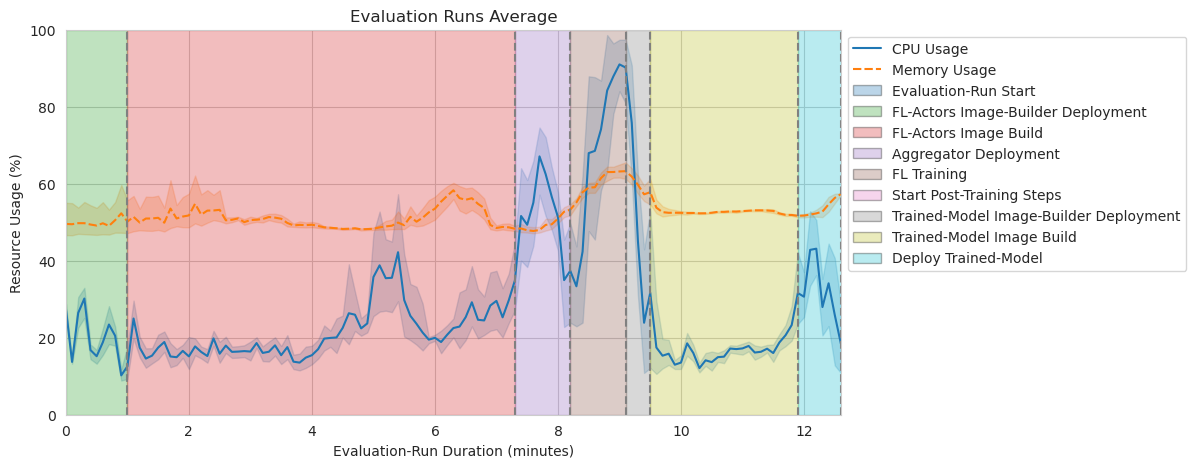
\includegraphics[width=0.95\paperwidth]{eval_1_simplest_cpu_mem.png}
        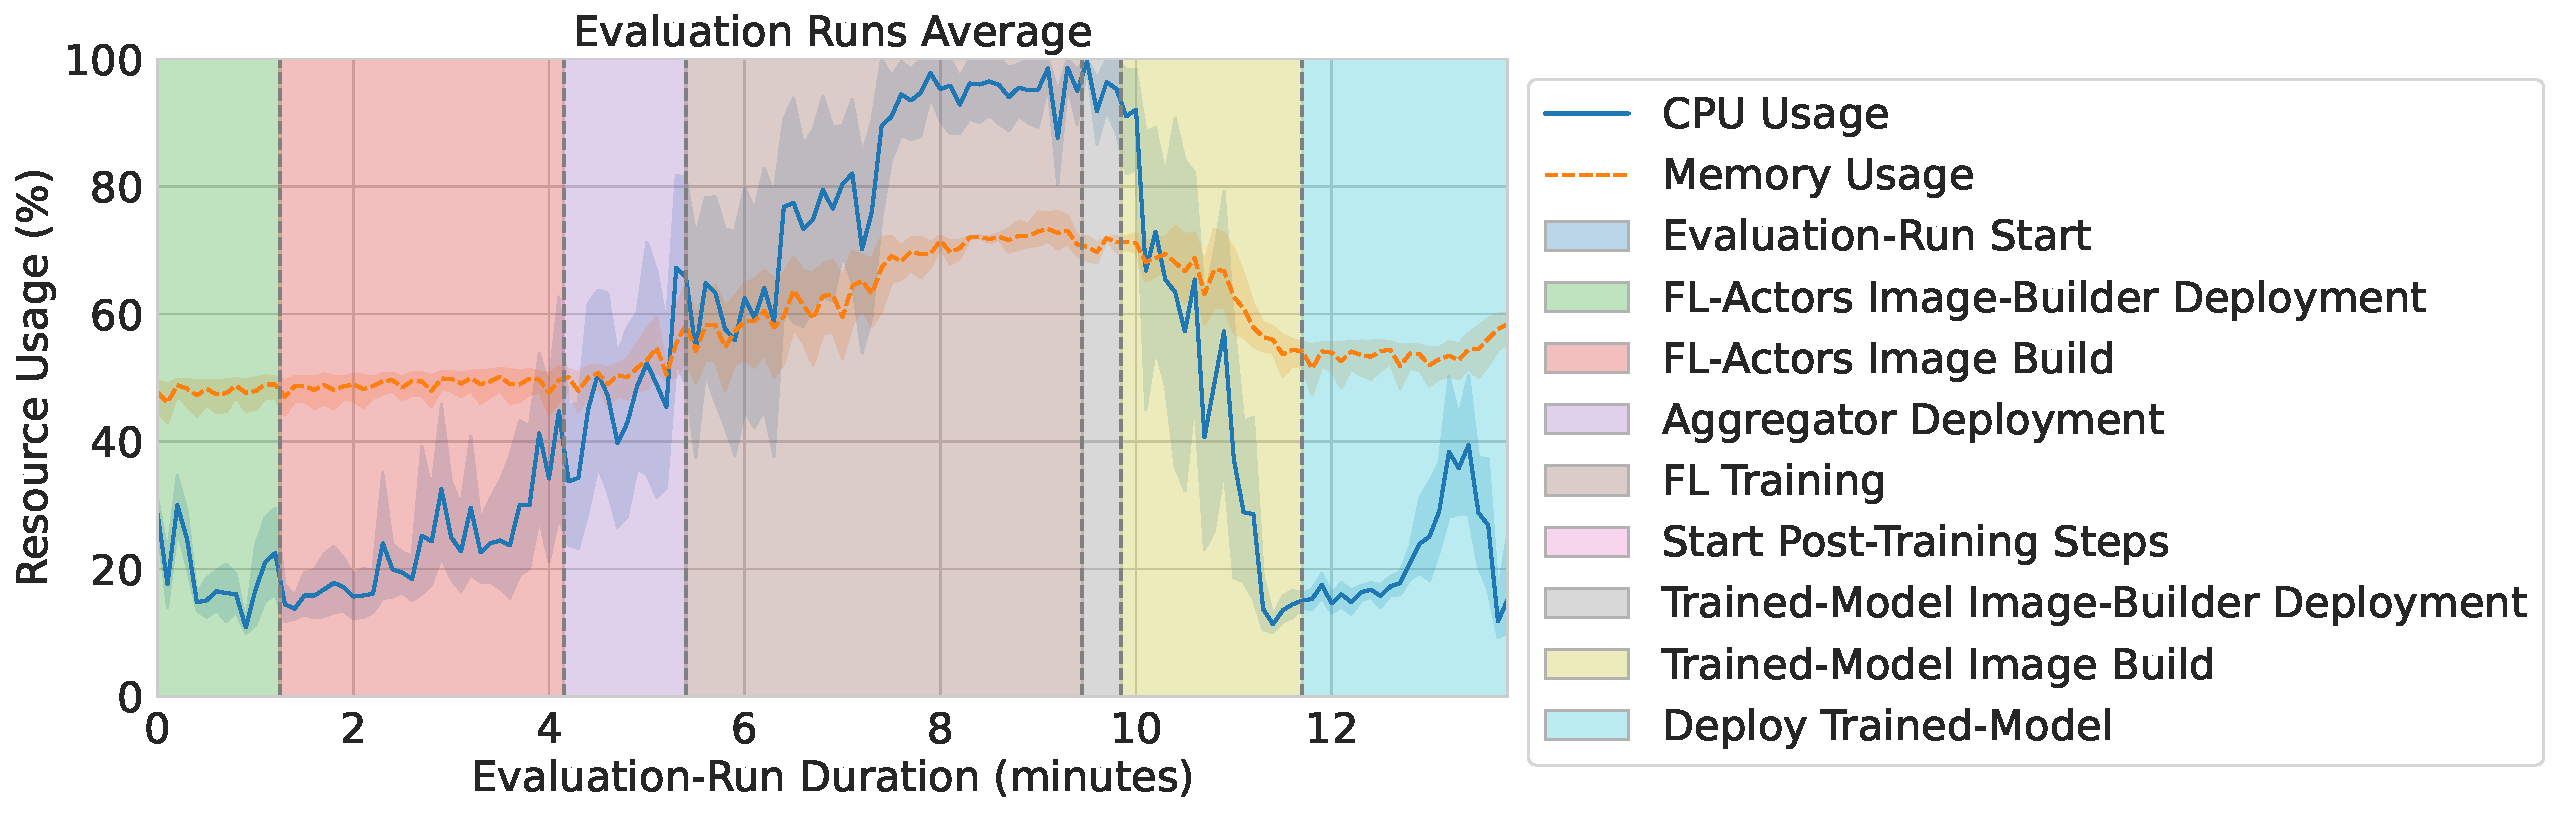
\includegraphics[width=0.95\paperwidth]{evaluations/experiment_1/cpu_mem.pdf}
        \caption{Experiment 1: CPU \& Memory Utilization}
        \label{fig:eval_1_simplest_cpu_mem}
    \end{adjustwidth}
\end{figure}

\begin{figure}[p]
    \begin{adjustwidth}{-0.2\paperwidth}{-0.2\paperwidth}
        \centering
        % 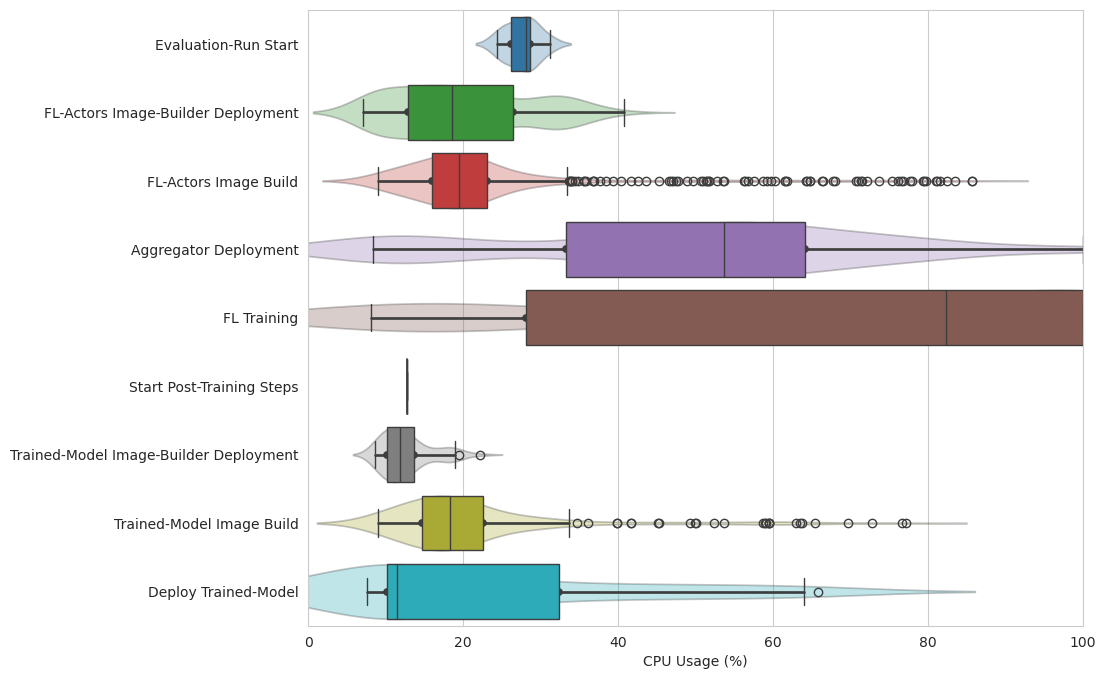
\includegraphics[width=0.70\paperwidth]{eval_1_simplest_cpu_boxviolin.png}
        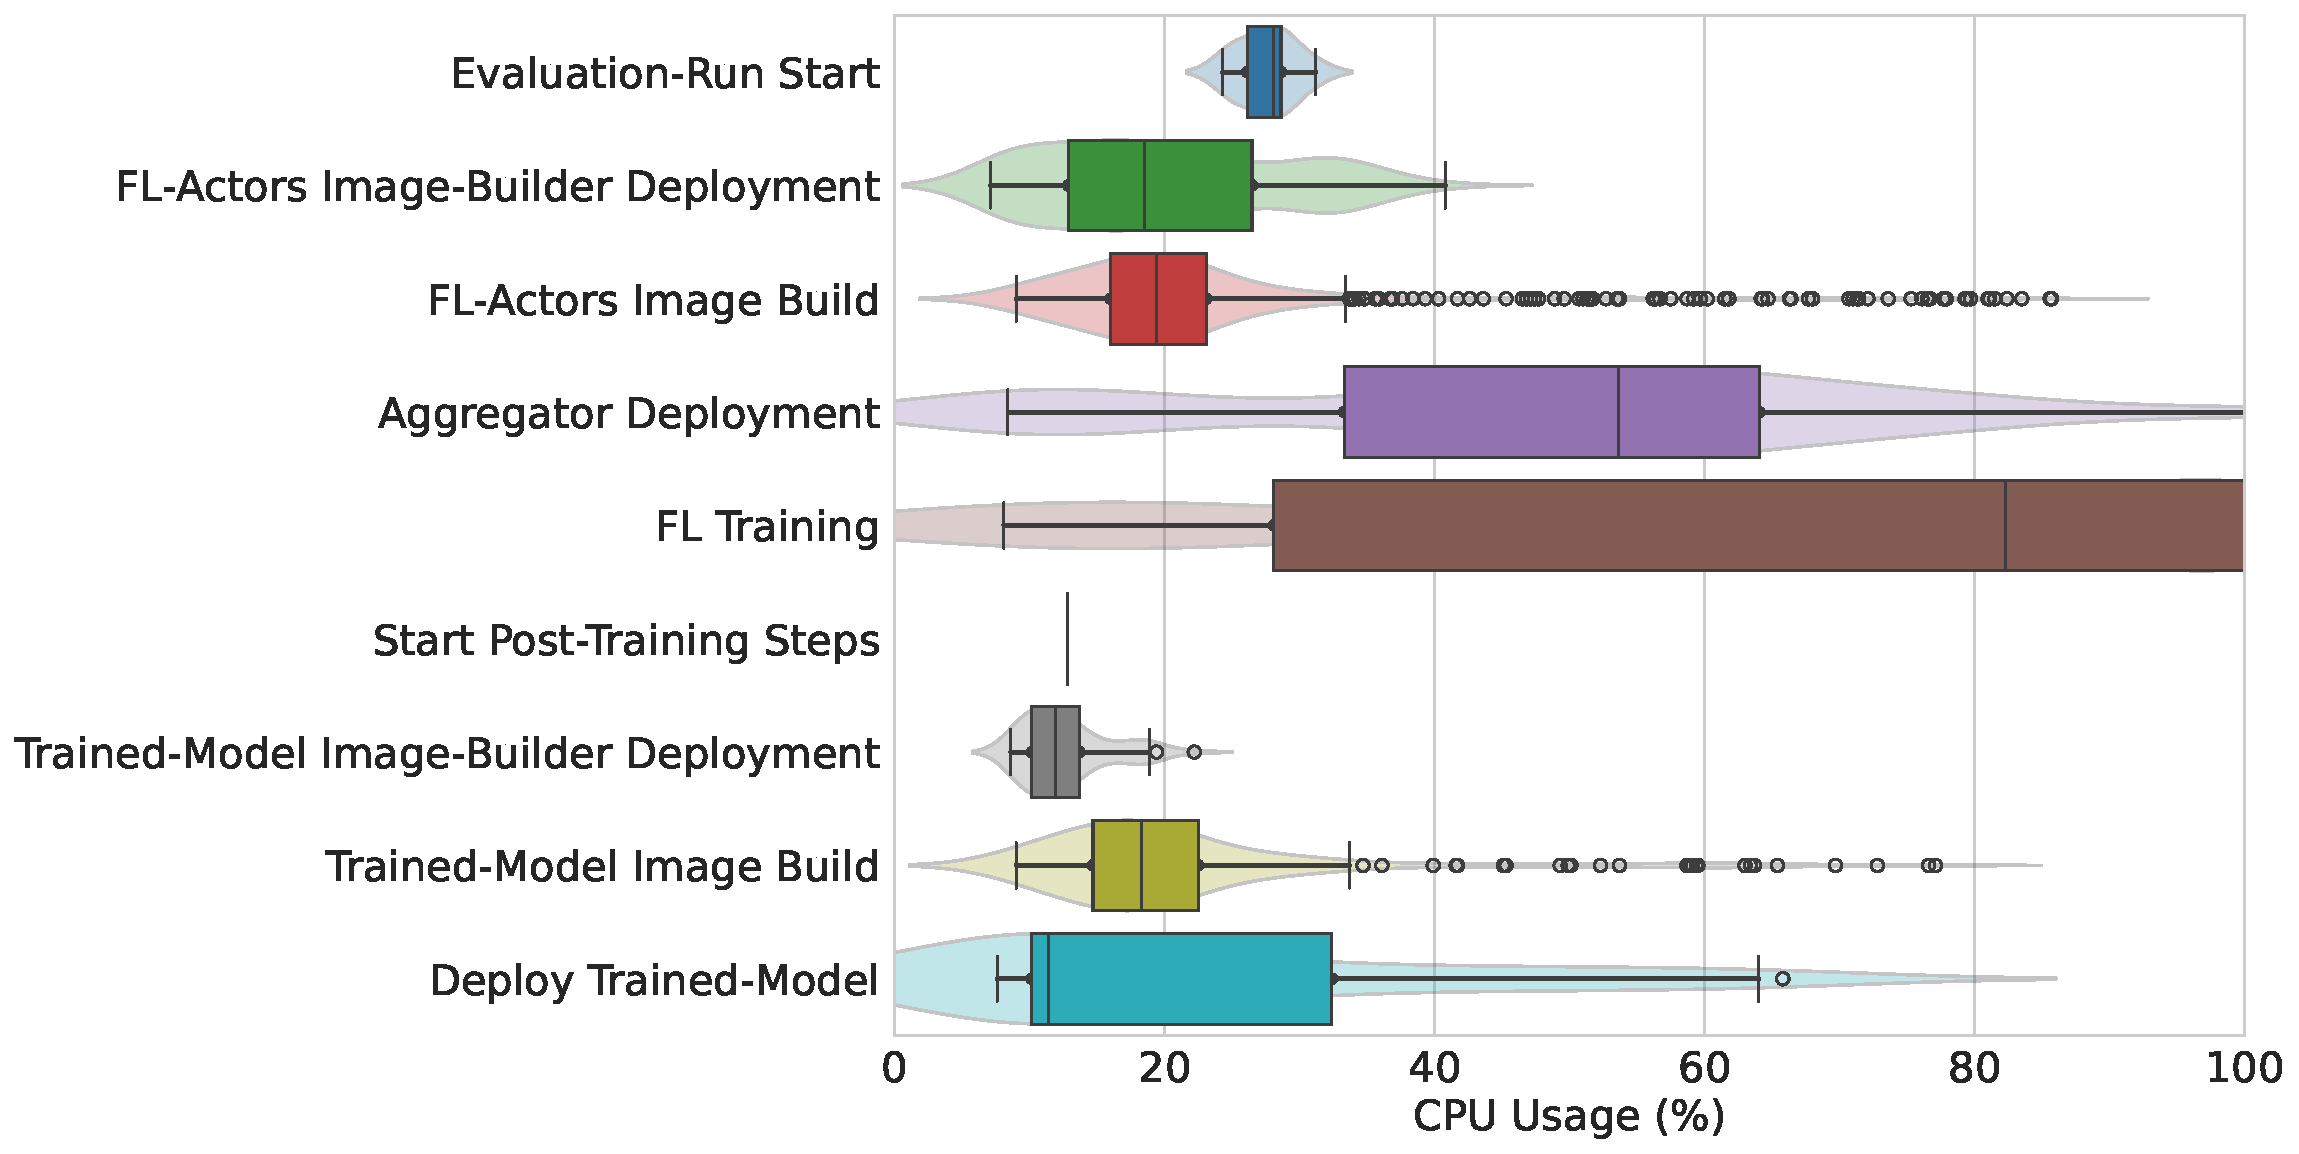
\includegraphics[width=0.85\paperwidth]{evaluations/experiment_1/cpu_by_stage.pdf}
        \caption{Experiment 1: CPU Utilization by Stage}
        \label{fig:eval_1_simplest_cpu_boxviolin}
    \end{adjustwidth}

    \begin{adjustwidth}{-0.2\paperwidth}{-0.2\paperwidth}
        \centering
        % 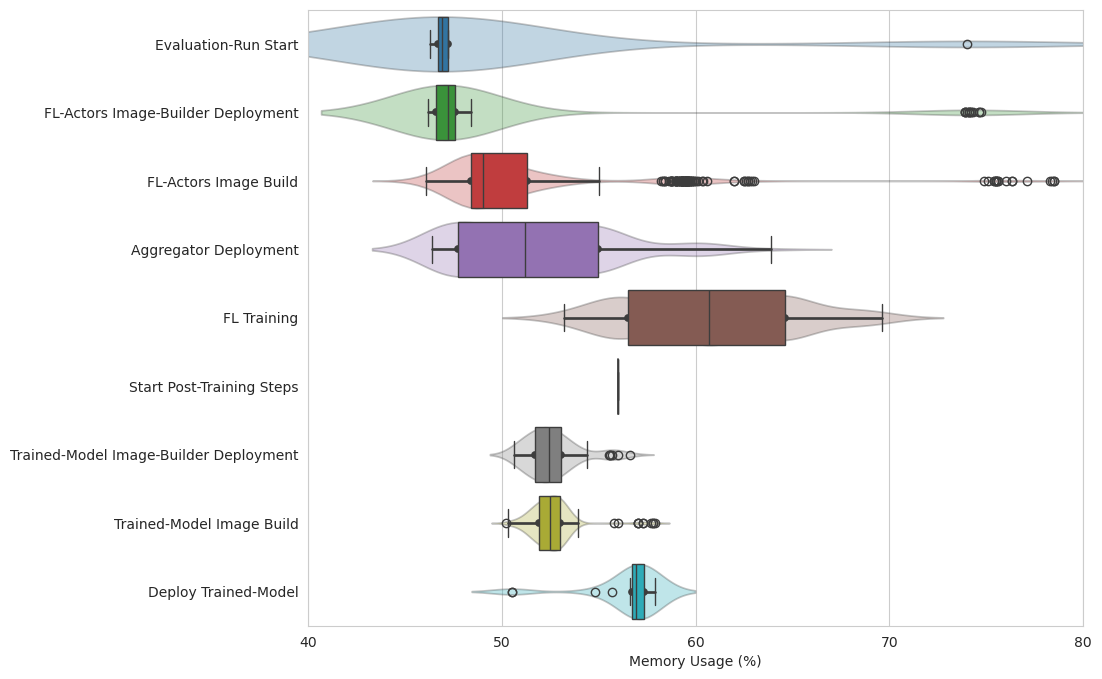
\includegraphics[width=0.70\paperwidth]{eval_1_simplest_memory_boxviolin.png}
        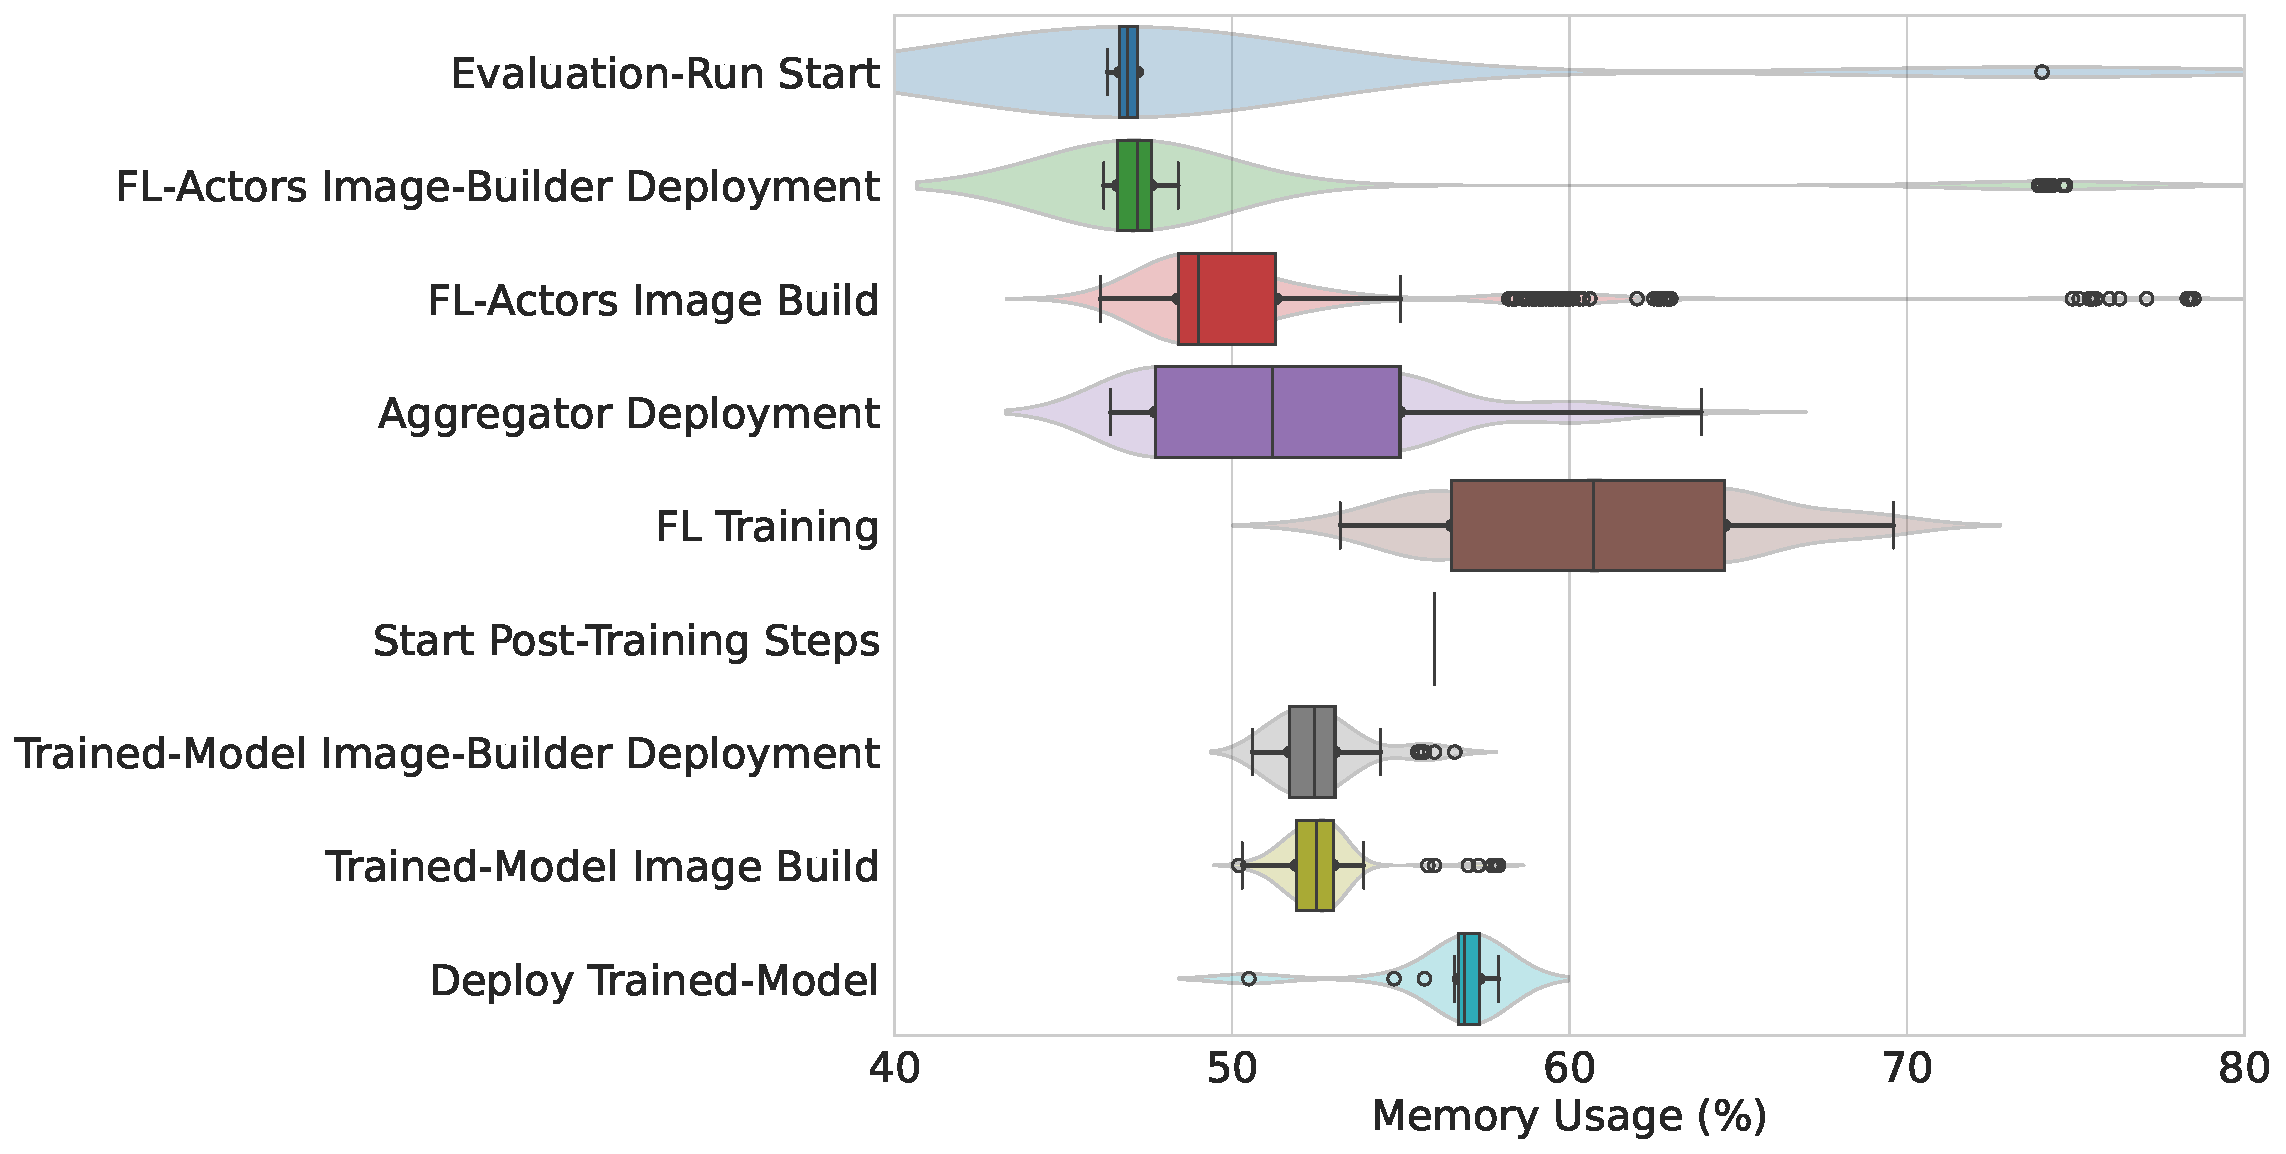
\includegraphics[width=0.85\paperwidth]{evaluations/experiment_1/mem_by_stage.pdf}
        \caption{Experiment 1: Memory Utilization by Stage}
        \label{fig:eval_1_simplest_memory_boxviolin}
    \end{adjustwidth}
\end{figure}

\pagebreak
\subsubsection{Normalization}

\begin{figure}[h]
    % \begin{adjustwidth}{-0.2\paperwidth}{-0.2\paperwidth}
        \centering
        % 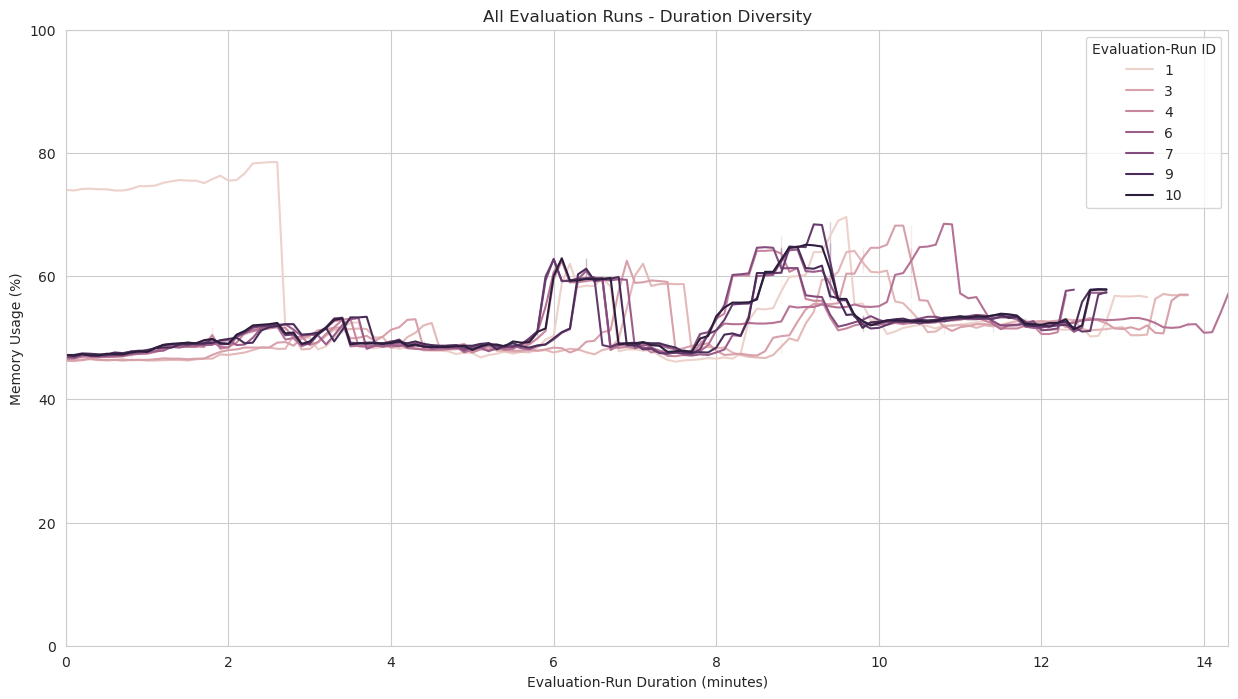
\includegraphics[width=0.99\paperwidth]{eval_1_simplest_explanation_shift.png}
        % 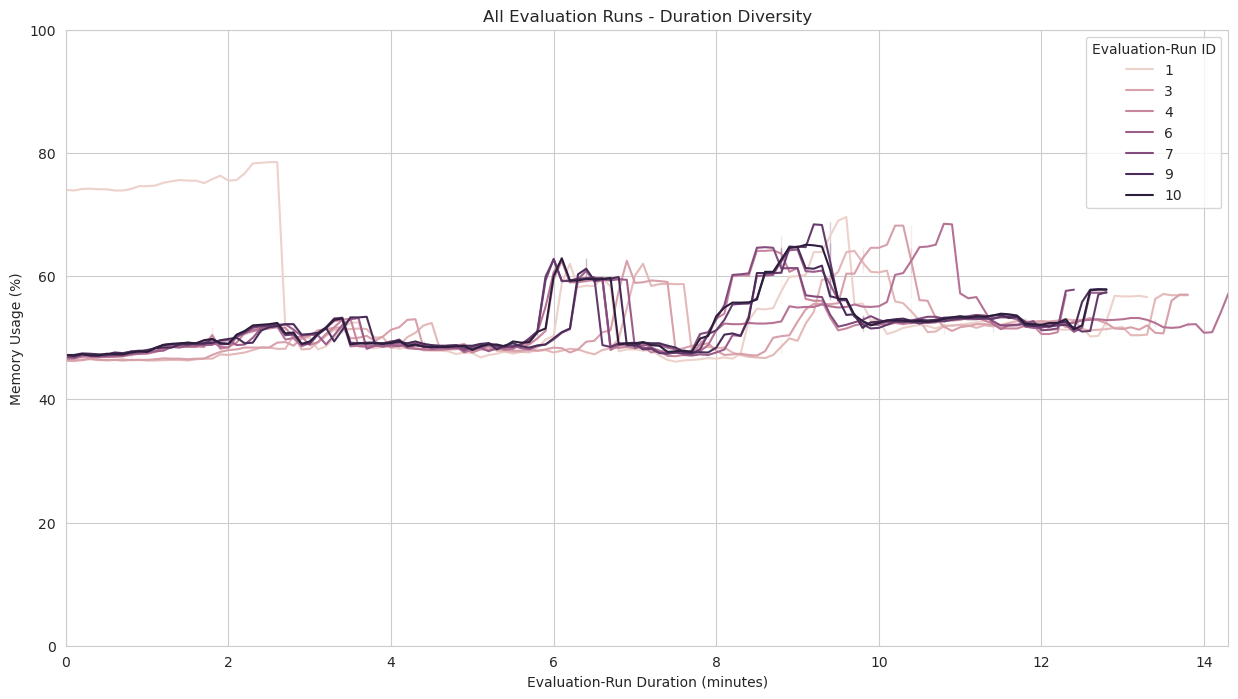
\includegraphics[width=1.0\textwidth]{eval_1_simplest_explanation_shift.png}
        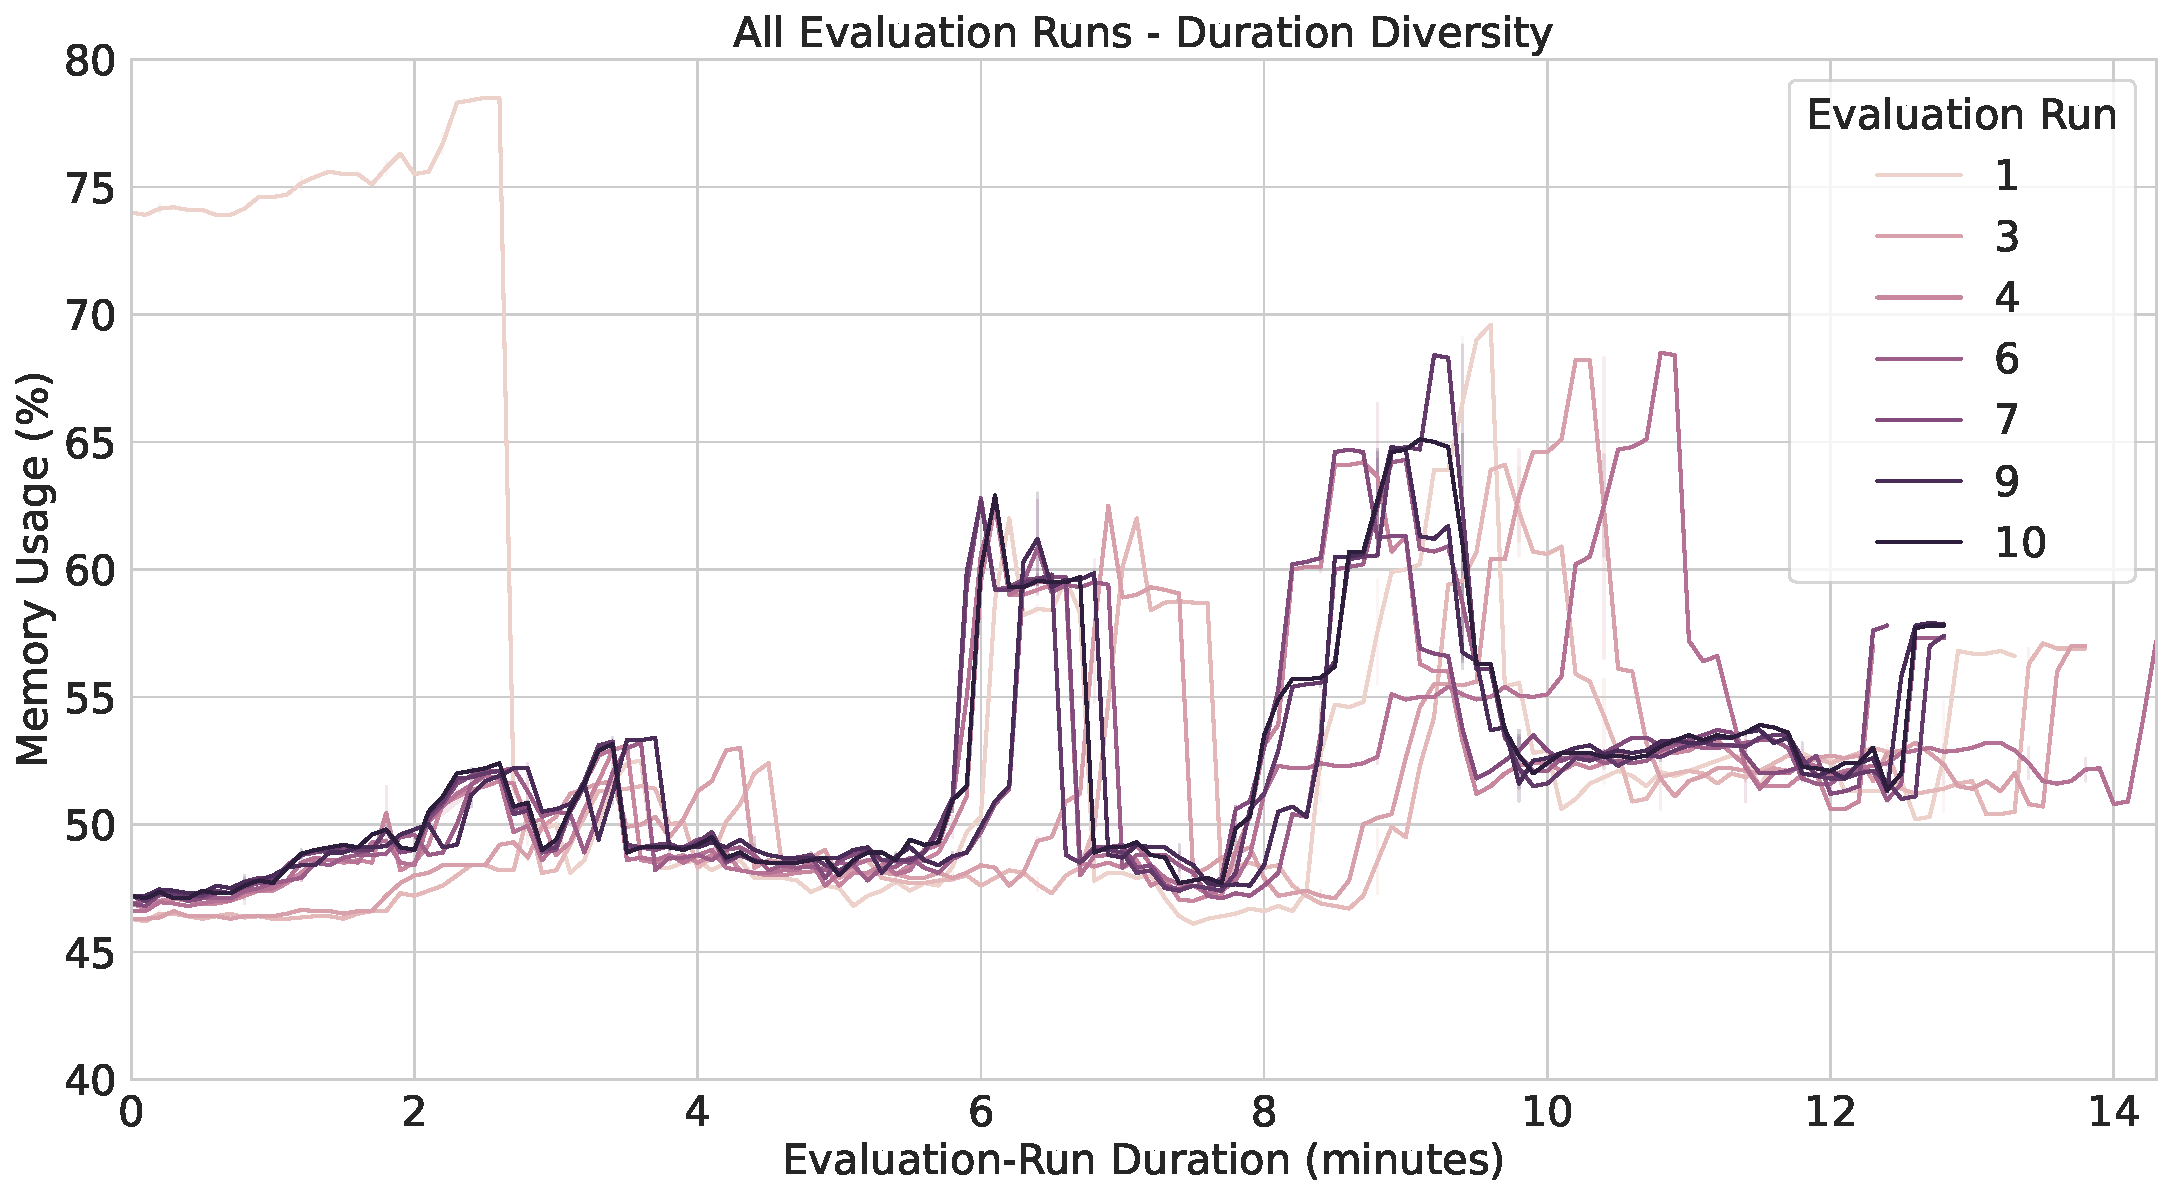
\includegraphics[width=1.0\textwidth]{evaluations/experiment_1/explanatory.pdf}
        \caption{Individual Experiment Memory Usage}
        \label{fig:eval_1_simplest_explanation_shift}
    % \end{adjustwidth}
\end{figure}

Individual evaluations range in duration.
The reasons for this can be manifold, such as different current image pull speeds due to local network conditions or remote registry loads.

Figure \ref{fig:eval_1_simplest_explanation_shift} shows the memory usage of individual evaluation rounds over time.
It is clear to see that the usage pattern is the same but shifted over time.
We normalized the average of these rounds to compare and visualize them properly.
Otherwise, stage borders become duplicated and overlapped, means and confidence intervals do not lead to meaningful outcomes, and the graphs are more confusing than helpful.

\subsubsection{Disk Space} \label{subsection:disc_space}

Graph \ref{fig:eval_1_simplest_disk_space} shows how the disk space changes over the project's lifetime.
There was a total average increase of 14 GB.
It starts with the Image-Builder-Deployment stage, where the Image-Builder image is pulled.
Many components and dependencies are downloaded and pushed to the registry on the same monolithic device during the FL actors' build process.
The jump in disk space in the aggregator (FL actors) deployment stage is because containerd needs to pull these build images.
Thus, the monolith will have the same image in the image registry and its local containerd image context.
During FL training, the disk space remains the same, which verifies that even when using FLOps with demanding lengthy training configurations and models, no disk space issues will arise due to its training process.
Disk space occasionally goes down due to the system's garbage collection, which is independent of FLOps or Oakestra.
The aggregator (FL-actors) deployment stage takes up the most space.
The trained-model image deployment stage is minimal compared to the first builder deployment because of the local containerd image storage.
Containerd pulls the builder image once and reuses it afterward.
This means that dedicated worker nodes that handle several project builds can pull these reoccurring images once and reuse them for all projects.
Especially during image-building processes, much space is freed up again due to garbage collection.

\begin{figure}[t]
    \begin{adjustwidth}{-0.2\paperwidth}{-0.2\paperwidth}
        \centering
        % 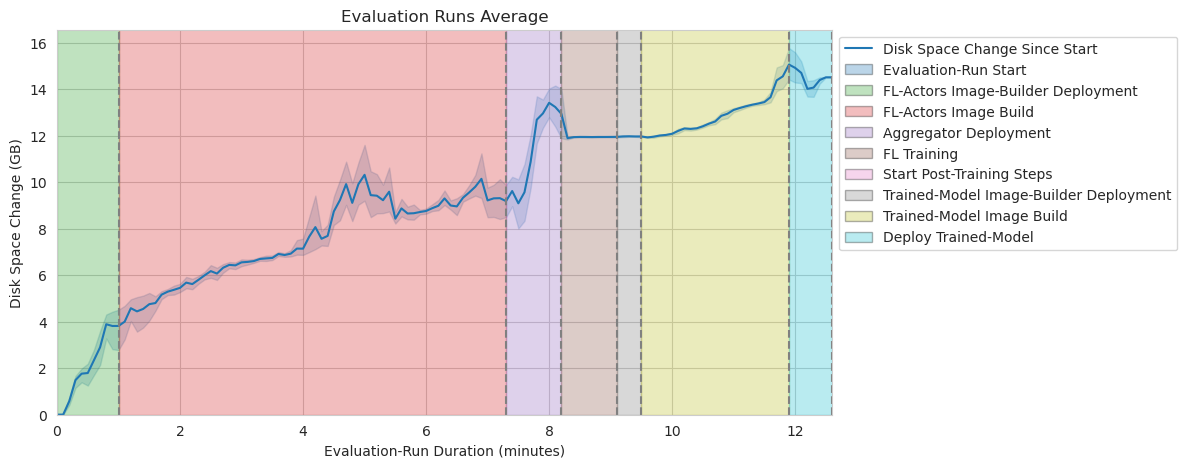
\includegraphics[width=0.99\paperwidth]{eval_1_simplest_disk_pace_linegraph.png}
        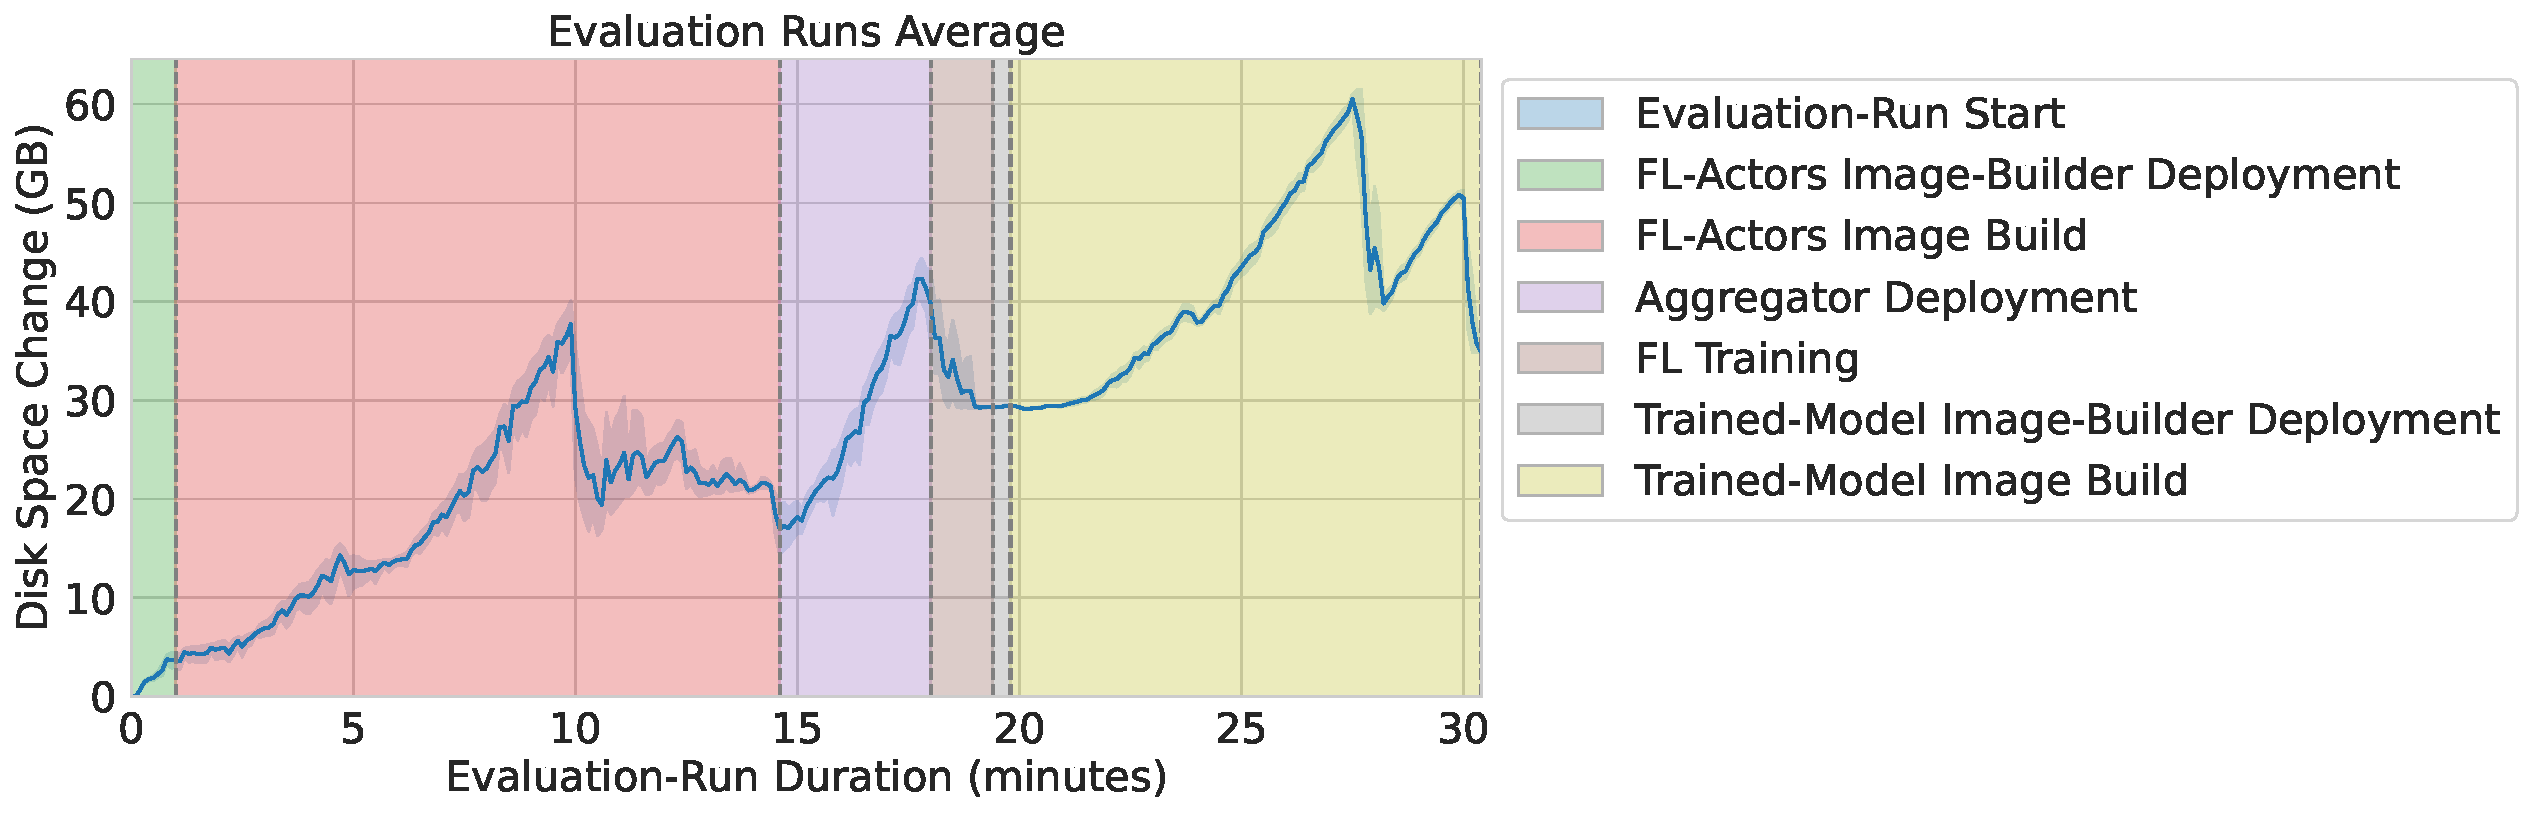
\includegraphics[width=0.99\paperwidth]{evaluations/experiment_1/disk_linear.pdf}
        \caption{Experiment 1: Disk Space Changes over Time}
        \label{fig:eval_1_simplest_disk_space}
    \end{adjustwidth}
\end{figure}

\subsubsection{Network IO}

\begin{figure}[h]
    \begin{adjustwidth}{-0.2\paperwidth}{-0.2\paperwidth}
        \centering
        % 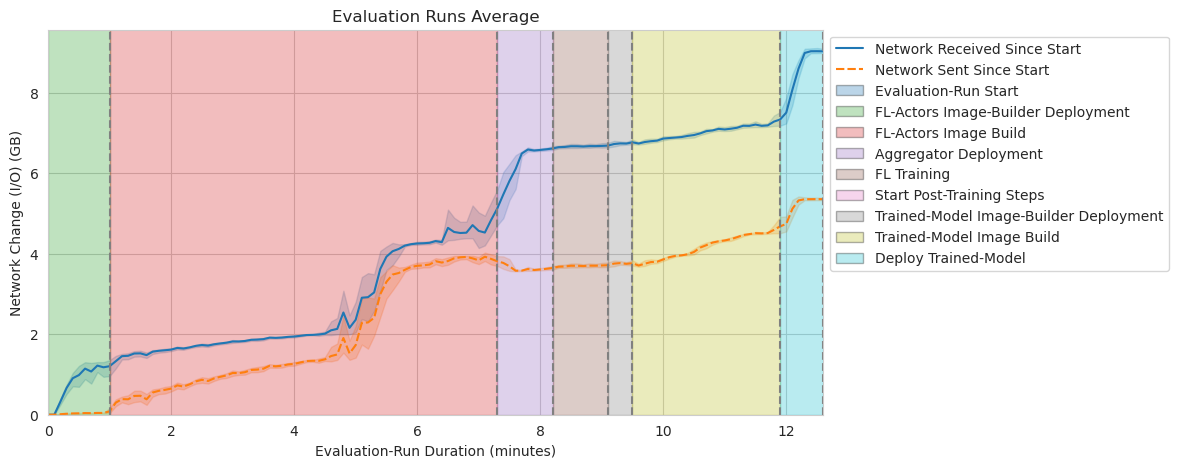
\includegraphics[width=0.99\paperwidth]{eval_1_simplest_network_linegraph.png}
        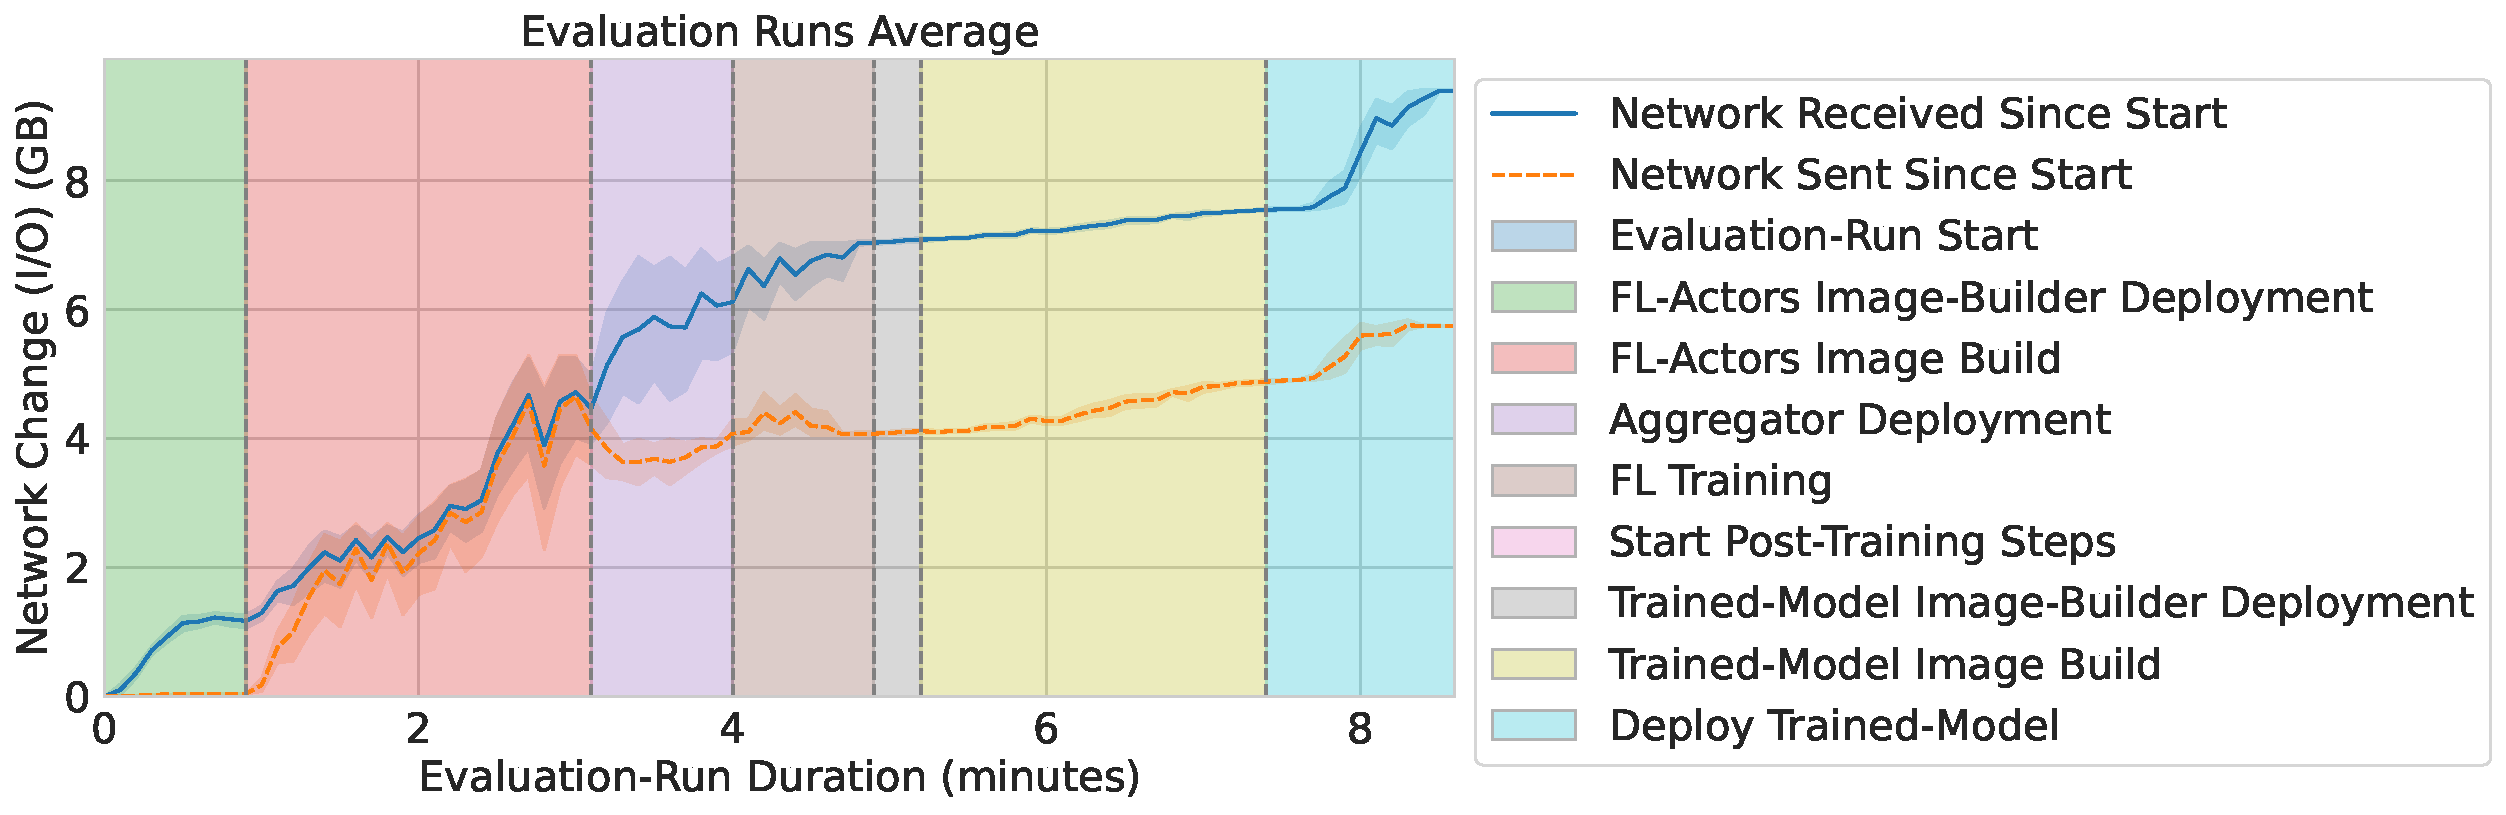
\includegraphics[width=0.99\paperwidth]{evaluations/experiment_1/net_io.pdf}
        \caption{Experiment 1: Net-IO over Time}
        \label{fig:eval_1_simplest_net_io}
    \end{adjustwidth}
\end{figure}

Figure \ref{fig:eval_1_simplest_net_io} shows the network loads received and sent over a project runtime.
The most significant increases are during built image pushes.
They occur around minute five when the base image is pushed, at the end of the FL-Actors Image Build stage phase, and when the trained-model image build stage bleeds into its deployment stage.
We omit to present further (violin-box) plots detailing net-IO because this additional information does not lead to any significant insights.

These values should be strictly increasing due to the accumulative nature of network IO counters.
This plot shows dips.
The reason for this is connected to removed containers.
The displayed lines are the sums of all received and sent traffic detectible on all network interfaces.
This includes virtual network interfaces of containers.
For example, there is a noticeable decrease between the FL-Actors image build and aggregator deployment stages.
I.e., between the moment the builder service finishes pushing its images and terminates and before these build services get deployed.
The image builder container had its own virtual network interface, which was included in the total sum and represented as a plotted line.
Once the container is removed, its virtual network interface is also deleted, and its accumulated net IO will be removed from the sum of the following system metrics scrapes.

\subsubsection{Stage Runtimes \& Training Results}
Figure \ref{fig:eval_1_simplest_stage_durations} shows each stage's average duration.
The FL training stage is relatively short because the training configuration is minimal.
The image build stages both take up the vast majority of time.
The FL-actors image build process involves more images with complex dependency resolutions.
Thus, this build stage takes over twice as long as the trained-model image build.
Figures \ref{fig:eval_1_simplest_accuracies} and \ref{fig:eval_1_simplest_loss} show the accuracies and losses of the trained models after each evaluation round.
They prove that FLOps can train ML models in a stable way.

\begin{figure}[H]
    \begin{adjustwidth}{-0.2\paperwidth}{-0.2\paperwidth}
        \centering
        % 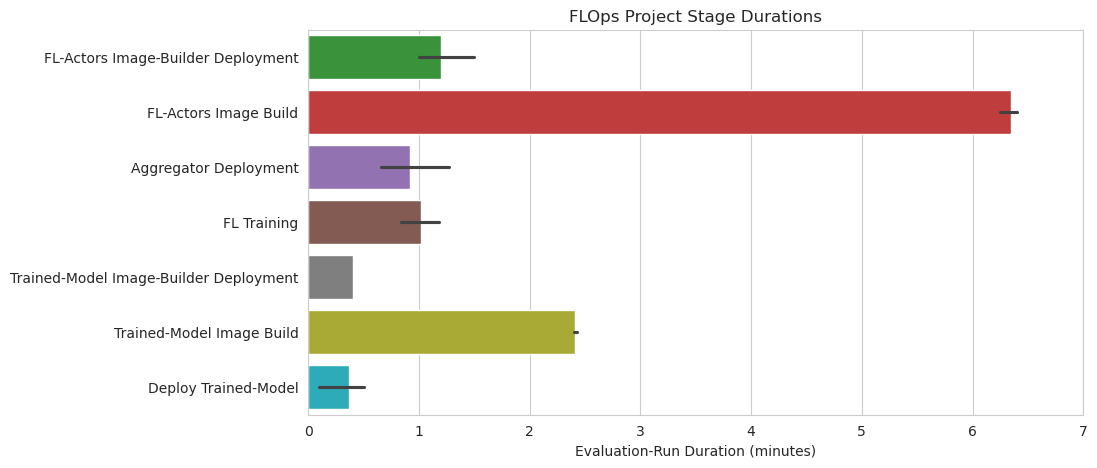
\includegraphics[width=0.80\paperwidth]{eval_1_simplest_stage_durations.png}
        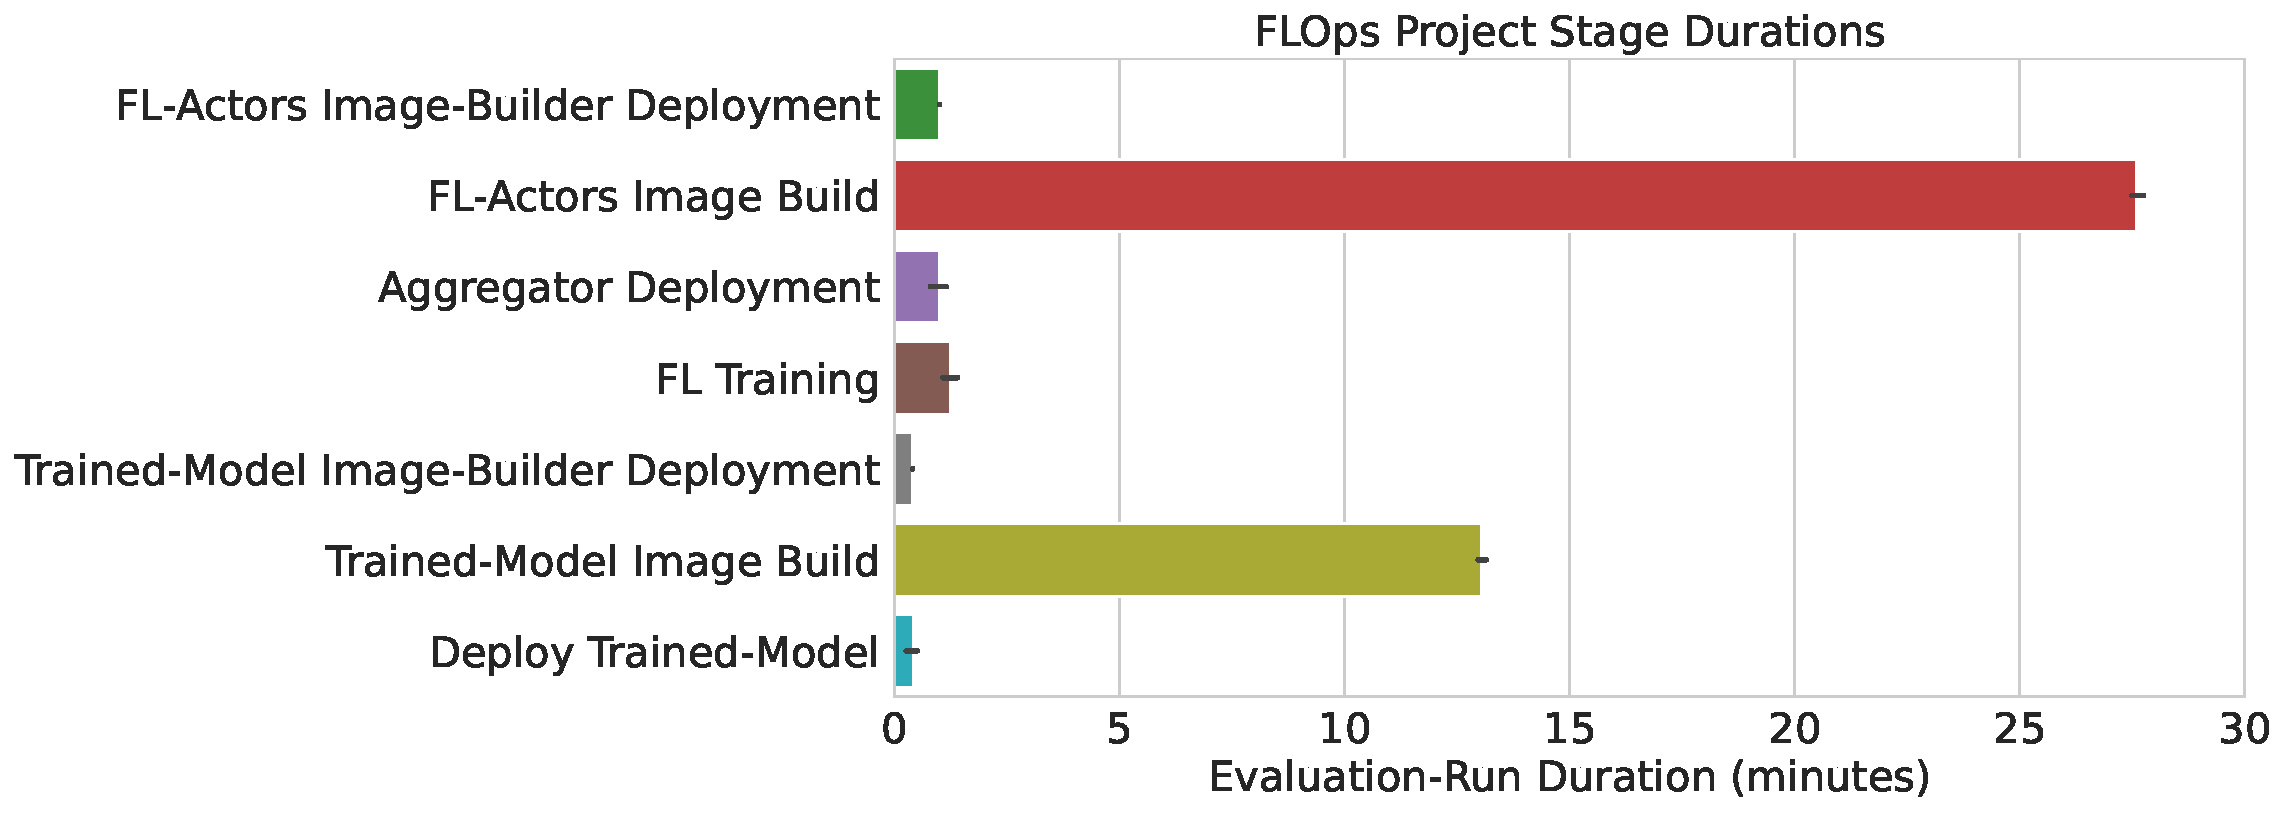
\includegraphics[width=0.90\paperwidth]{evaluations/experiment_1/stage_durations.pdf}
        \caption{Experiment 1: Stage Durations}
        \label{fig:eval_1_simplest_stage_durations}
    \end{adjustwidth}
\end{figure}

\begin{figure}[H]
    \centering
    % 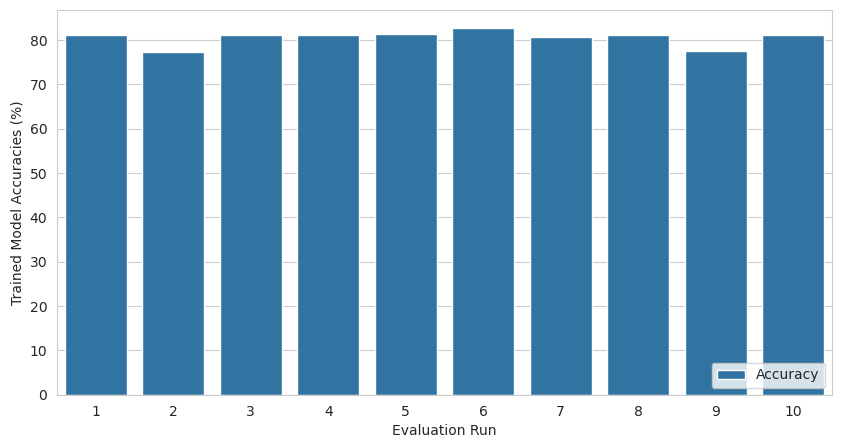
\includegraphics[width=0.90\textwidth]{eval_1_simplest_accuracy.png}
    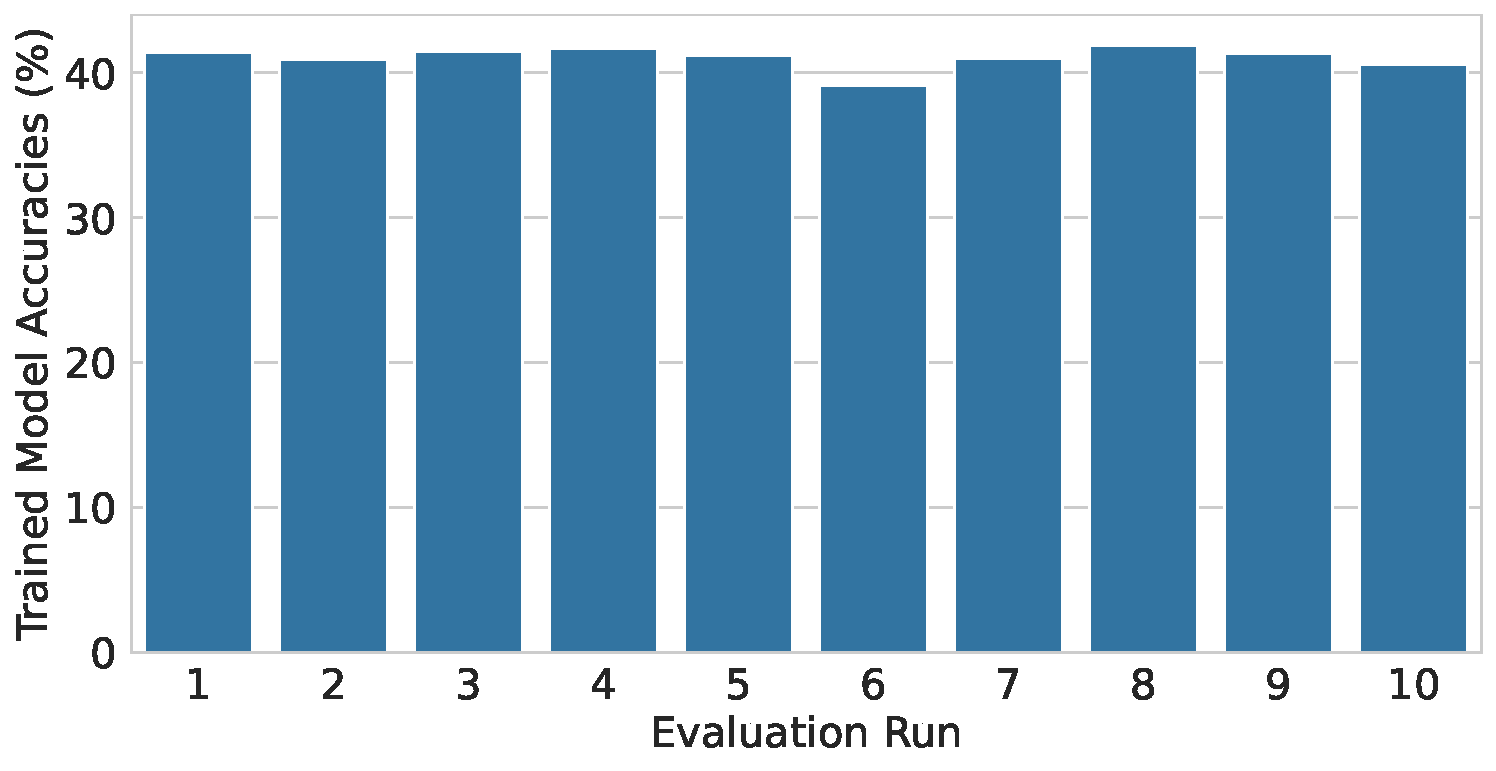
\includegraphics[width=0.90\textwidth]{evaluations/experiment_1/accuracy.pdf}
    \caption{Experiment 1: Trained Model Accuracies}
    \label{fig:eval_1_simplest_accuracies}
\end{figure}

\begin{figure}[H]
    \centering
    % 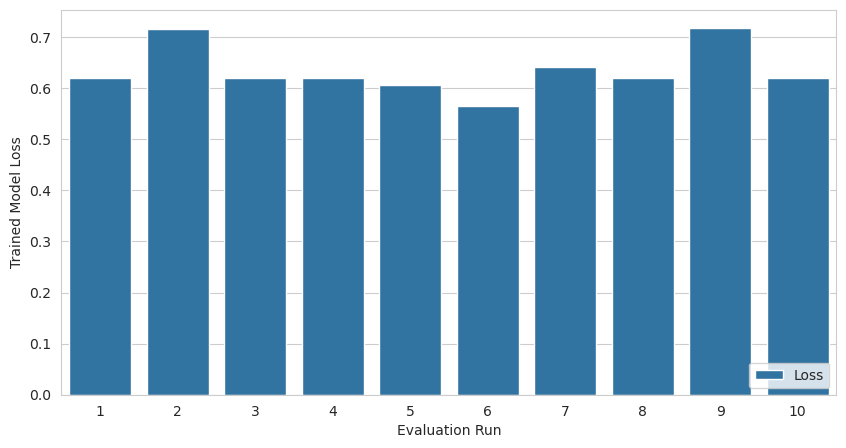
\includegraphics[width=0.90\textwidth]{eval_1_simplest_loss.png}
    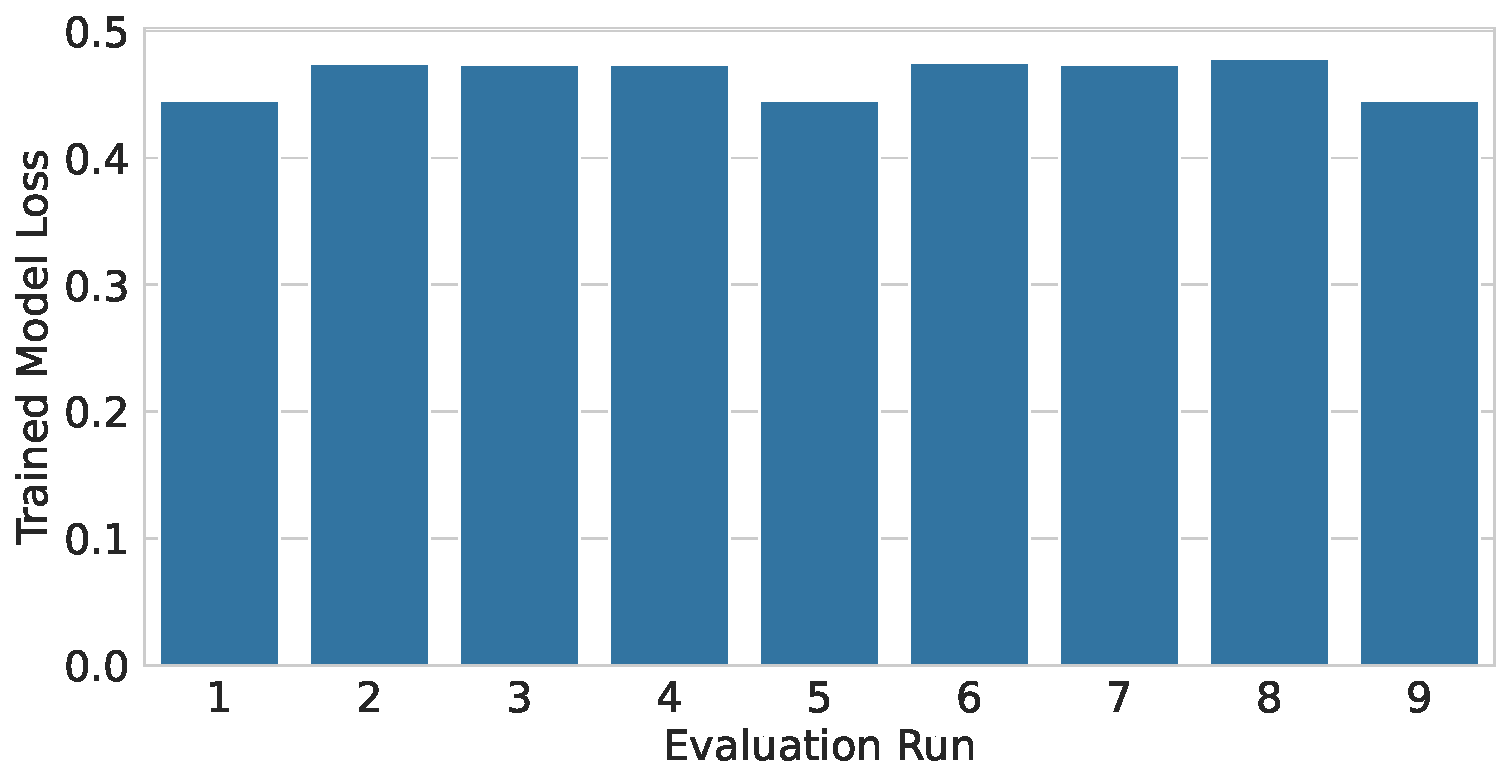
\includegraphics[width=0.90\textwidth]{evaluations/experiment_1/loss.pdf}
    \caption{Experiment 1: Trained Model Loss}
    \label{fig:eval_1_simplest_loss}
\end{figure}

